%!TEX root = ../data-imputation.tex
\section{Results}
\label{sec:results}

In this section, we describe and visualize the results of our experiments. For the visualization we choose to consistently use boxplots for all four experiments/scenarios. These allow us to get a decent impression of the distribution of the results based on quantiles. In a line chart, in contrast, the confidence bands would overlap too much to derive meaningful interpretations. The plots' arrangement from left to right corresponds to the degree of difficulty increasing in this direction. This applies to the missingness patterns (MCAR, MAR, MNAR), each of which gets an own sub-plot, as well as the missingness percentages (small to larger), which are depicted as ticks on the x-axis. Due to mostly different results, we further distinguish the plots between regression and classification tasks. These are strongly imbalanced, with only 13\% of the results based on categorical columns (637) versus a clear majority of 87\% numerical columns (4293).


\subsection{Experiment 1: Imputation Quality}

In this experiment we evaluate the imputation performance of each method when training on fully observed data and incomplete data.

As described above, our goal was to provide a broad overview of the performance of different imputation methods on various data sets. It was difficult to compare the results across such heterogeneous data by their respective scores (F1/RMSE) on randomly sampled target columns. Therefore, we decided to use ranks instead. On each experiemental condition (see Table \ref{tab:experiment_settings}), we calculate the rank of every imputer based on its mean performance over three repetions (different random train-test splits). Since we have six imputers, there are six ranks, with one being the best and six being the worst. For numerical columns the rank is based on RMSE where lower is better and for categorical columns the rank is based on the F1 score where higher is better. Imputation methods with equal performance are assigned the same rank. If an imputation method did not work, it is ranked last.


\subsubsection{Scenario 1: Training on Complete Data}

\begin{figure}\centering
    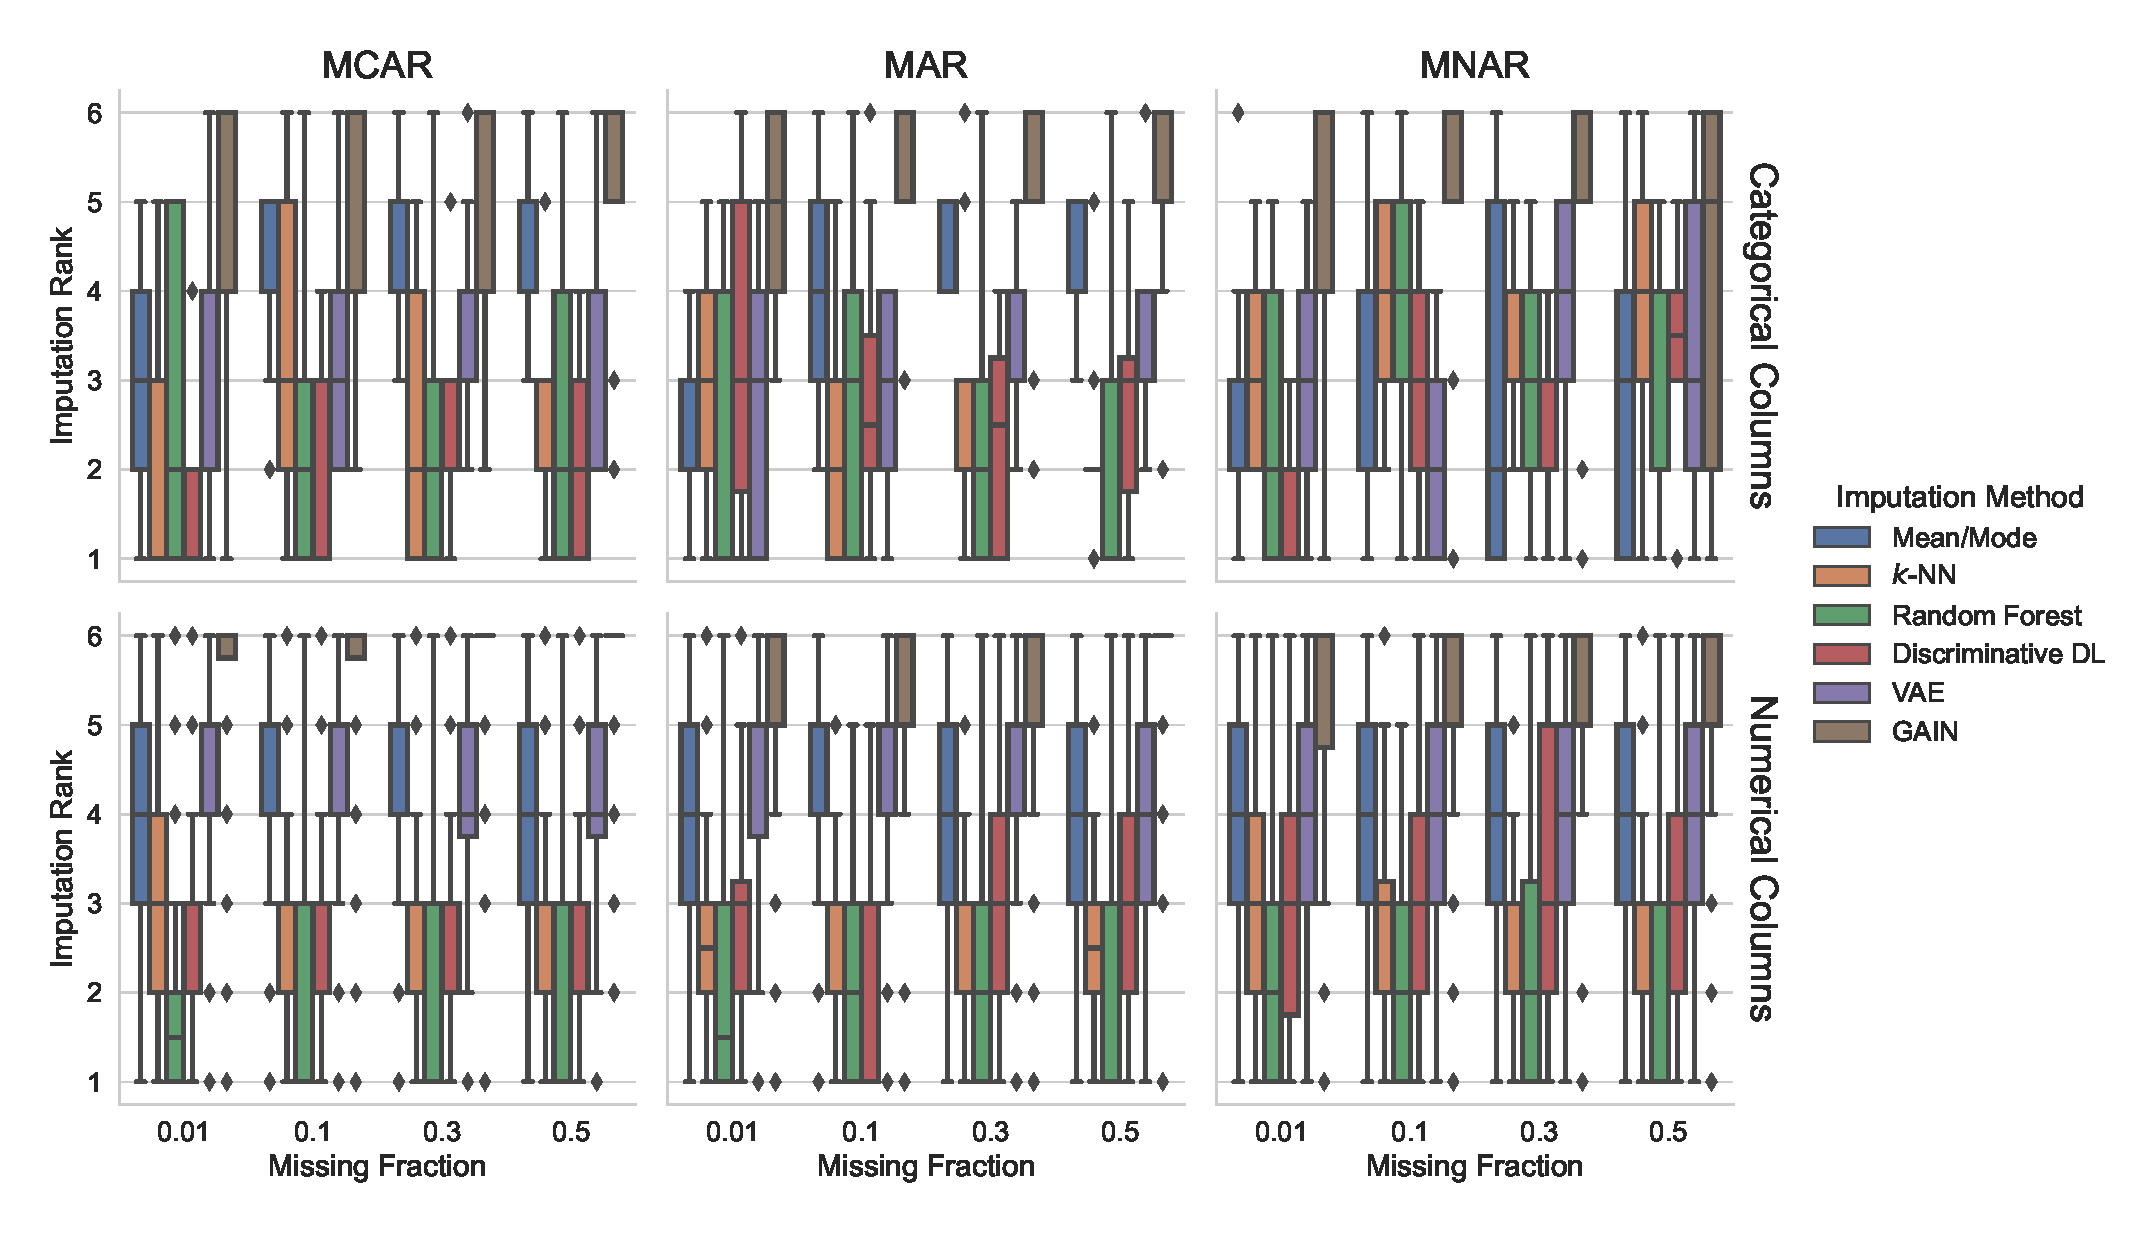
\includegraphics[width=1\columnwidth]{fully_observed_impute_rank_boxplot.eps}
    \caption[Imputation Ranks - Fully Observed]{Imputation quality of the six imputation methods trained on complete data. We plot the imputation method's rank against the missingness fraction. The columns of plots separate the changing missingness pattern, whereas the rows distinguish the results between categorical and numerical target columns. ML methods and discriminative DL tend to perform best. From left to right, we observe more variance (larger boxes), indicating that the results are less clear. Especially for categorical columns with the MNAR pattern and higher missingness fractions, mean/mode seems to be a good alternative.
	}
	\label{fig:fully_observed_impute_rank_boxplot}
\end{figure}

Figure \ref{fig:fully_observed_impute_rank_boxplot} shows the aggregated ranks for imputation performance when imputation methods are trained on fully observed data.

When imputing categorical columns, there is no clear winner. However, the Discriminative Deep Learning approach yields high imputation quality in most cases. In the MAR setting, also the methods random forest and $k$-NN are among the first two to three ranks often times. With increasing complexity the DL based methods seem to improve. Notably Mean/Mode imputation compares favorably in many cases especially in the most complex MNAR setting. Surprisingly, GAIN appeared to perform worse than others in most cases \sebastian{why? - explain that it fails very often (how many percents?)}. In the setting of highest complexity (MNAR with 50\% missing values) the results are not significantly worse than the other methods \sebastian{Gefährlicher Satz wegen significantly.. würde ich weg lassen}.

When imputing numerical columns the differences are more pronounced. Random Forest is the only method with 50\%\sebastian{$75\%$!! - box zeigt 25 und 75 quantile} of values\sebastian{meaning data sets - maybe better to make this clear} among the first three ranks throughout all experimental conditions. However, the whiskers indicate that there are also some results ranging on the middle and even last ranks. $k$-NN and Discriminative DL are almost as strong with the boxes indicating many second and third ranks, with k-NN performing a bit better \sebastian{Vll so: In most settings, KNN ranks in $50\%$ of the data sets as second or third with tendencies to better ranks.}. Mean/Mode and VAE are in the middle with the former in being slightly in the lead. \sebastian{Bisschen seh umgangsprachlich: Mean/Mode and VAE's ranks are similarly distributed over all ranks with tendency to the worse ranks. For easier settings, such as MCAR and MAR with smaller missingness fractions, Mean/Mode tends to be better than VAE.} Again, GAIN performs worst, this time even more clearly.

To summarize, classical ML methods and discriminative DL perform best when imputing missing values. However, for categorical columns there is often no improvement over Mode imputation \sebastian{Das ist gefährlich.. }. The generative methods are mostly outperformed even by Mean/Mode with VAE not as clearly as GAIN.


\subsubsection{Scenario 2: Training on Incomplete/Imputed Data}


\begin{figure}\centering
    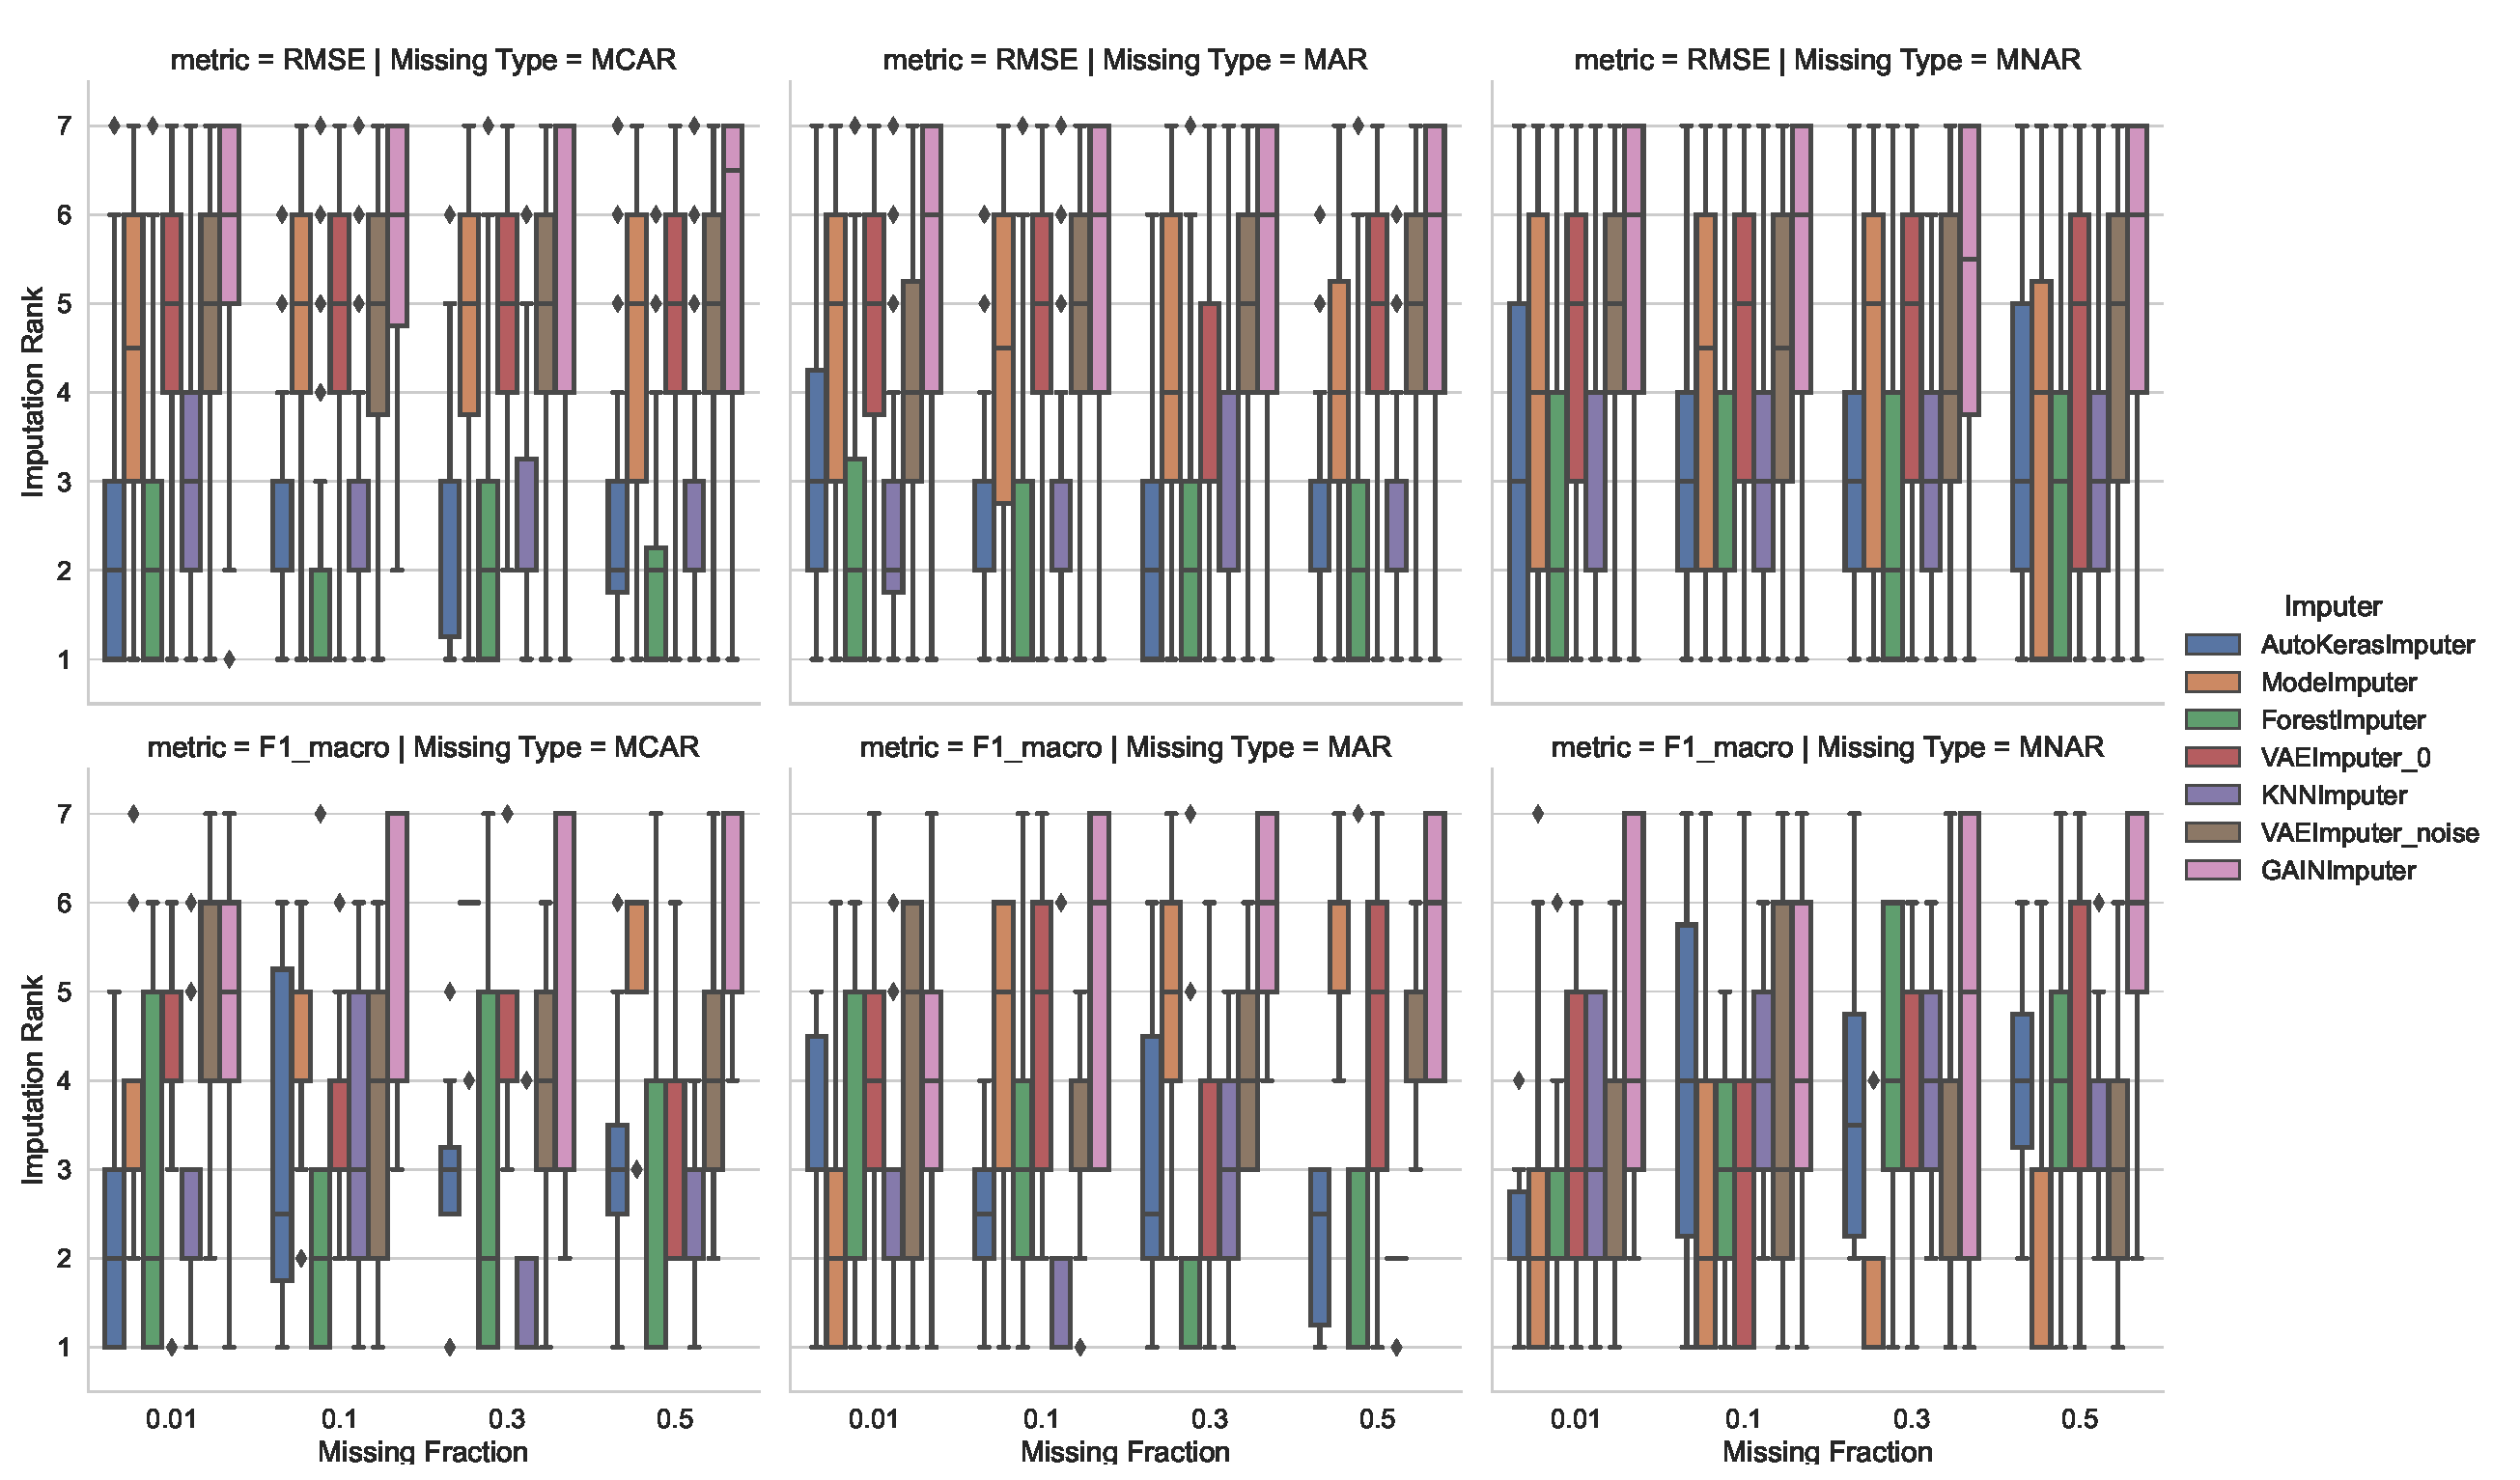
\includegraphics[width=1\columnwidth]{corrupted_impute_rank_boxplot.eps}

    \caption[Imputation Ranks - Corrupted]{Imputation quality of the six imputation methods trained on incomplete/imputed data. We plot the imputation method's rank against the missingness fraction. The columns of plots separate the changing missingness pattern, whereas the rows distinguish the results between categorical and numerical target columns. ML methods and discriminative DL tend to perform best. However, for categorical columns in the MNAR setting, there is often no improvement over mode imputation. \arndt{@Sebastian: ich finde, den letzten Satz kann man schon so schreiben im Bezug auf MNAR. Oder würdest du den weglassen?}
    }
	\label{fig:corrupted_impute_rank_boxplot}
\end{figure}

\autoref{fig:corrupted_impute_rank_boxplot} shows the imputation performance in \textit{Scenario 2}, i.e. when training on incomplete/imputed data\sebastian{Nur incomplete. Imputed haben wir nicht gemacht..}. For categorical columns it is even harder to find clear patterns. With increasing task difficulty, the performance\sebastian{Nicht performance der rank} of the Mean/Mode imputation increases, though with higher variance. Interestingly, Mode imputation outperforms other methods especially in the most challenging settings (MNAR with 30\% and 50\% missing values)\sebastian{Spätestens jetzt sollten wir mal ein wort darüber verlieren woran das liegen könnte: When eine category einfach häufiger ist, dann ist das meist ne recht guter guess. Das könnte dazu führen, dass die andere schlechter werden, weil die versuchen das intelligenter zu machen, aber einfach nicht genügend trainings daten haben um noch was sinnvolles zu lernen}. The methods $k$-NN and random forest compare favorably in the MCAR and MAR setting, but random forest has much higher variance. Discriminative DL yields similar performance in these settings, slightly worse on average and with lower variance than random forest. For MCAR and MAR these three methods tend to yield better performance than using Mean/Mode imputation, especially with an increasing fraction of missing values. The generative models tend to perform worst, especially GAIN.

Similar to the fully observed training case \sebastian{link to section}, imputation on numerical columns yields a clearer ranking than for categorical missing values. The imputation models $k$-NN and random forest yield best performances with a tendency of random forest to outperform $k$-NN, with larger variance of random forest. The Discriminative DL approach yields similar performance to the classical ML approaches in the MCAR and MAR settings. In the more challenging MNAR setting it performs slightly worse. Mean imputation and VAE perform comparably but worse than k-NN and Random Forest. GAIN falls on the last rank in most cases also in this setting.

Overall, the results of \textit{Scenario 1} (Figure \ref{fig:fully_observed_impute_rank_boxplot}) and \textit{Scenario 2} (Figure \ref{fig:corrupted_impute_rank_boxplot}) for numeric columns are quite similar. GAIN has become somewhat better in Scenario 2, although it still ranks worst. For categorical columns, the visualizations of the two scenarios are more pronounced in the incomplete training data setting. However, there are no major shifts in which the median worsens by more than two ranks. \arndt{Die letzte Aussage müssten wir prüfen, das geht aus den Plots nicht eindeutig hervor.}\sebastian{Würde das noch gröber halten:
\begin{itemize}
	\item Ob imputation methods auf complete oder incomplete trainiert sind macht an den ranks im großen und ganzen kein unterschied
	\item Schwierigere probleme (pattern oder fraction) machen ergebnisse weniger eindeutig (größere variance)
	\item Classische ML methoden:$k$-NN and random forest sind meist ne ziemlich gute wahl dicht gefolgt von Mean/mode, vor allem wenn probleme komplexer werden oder data incomplete sind (könnte daher kommen, dass eben dann das lernen schwerer wird.)
\end{itemize}
}

We attribute the poor performance of GAIN in part to its numerical instability. Out of our 828 runs per imputation method GAIN failed 273 times, which amounts to 33\% of the cases. In those cases GAIN was assigned the last rank. \sebastian{Ah ja, das würde ich nach oben schieben.. Und vll nicht sagen, dass es "numerical unstable" is ohne dass wir genauer rein geschaut haben..}

\subsubsection{Conclusions}
\felix{conclusions should be in the conclusions section, i guess?}
\arndt{nur eine temporäre sammlung von ideen}

- higher variance of random forest over knn due to outliers ?!

- generative methods mostly worse than mean/mode

- discriminative often as good as classical ML and better than mean/mode, but when considering the runtime might not be a good choice



\subsection{Experiment 2: Impact on Downstream Task}

In this experiment we evaluate the downstream performance of each method when training on fully observed data and incomplete data.

In \textit{Scenario 1} we use the definition for \textit{impact on downstream task} from \autoref{eq:impact}. In contrast, for \textit{Scenario 2} we use the slightly different definition from \autoref{eq:impact_scenario2}. Both of theses metrics are labeled \textit{Improvement} and the values represented on the Y-axis in \autoref{fig:fully_observed_downstream_boxplot} and \autoref{fig:corrupted_downstream_boxplot}.

\sebastian{Würde auch hier erst eine allgemienere einführugnen machen: Zeigen hier die Improvement berechnert wie in equation 3 o. 4 depending on scenario. Dass wir jetzt oben Classificaiton tasks und unten Regression haebn... UND: vor allem muss hier hien, dass wir jetzt nur noch die verwenden, die auch wirklich sinnvolle ergebnisse geliefert haben, also bein GAIN einiges fehlt.}

\felix{we should highlight the limitations of our results (only one column, maybe too simple)}


\subsubsection{Scenario 1: Training on Complete Data}

\sebastian{GANZ WICHTIG: wir haben hier keine infos darüber, welche columns imputed wurden. Was wir sehen ist ne Gruppierung nach Downstream task! - Ich würde da noch etwas weiter raus zoom am anfang: Allgemien, mehr missingness fürht zu mehr variance in der improvement. Überraschenderweise für calssification in beide Richtugnen aber deutliche tendenz für improvement und wieder wie oben RF/KNN/DL und Mean/mode sind ganz gut.. Regression fast ausschließlich improvements und wieder das bekannte trio am besten im regelfall.. (Hbane wir ne idee warum classificaiotn auch schelcht wird und regression nicht?)}


\begin{figure}\centering
	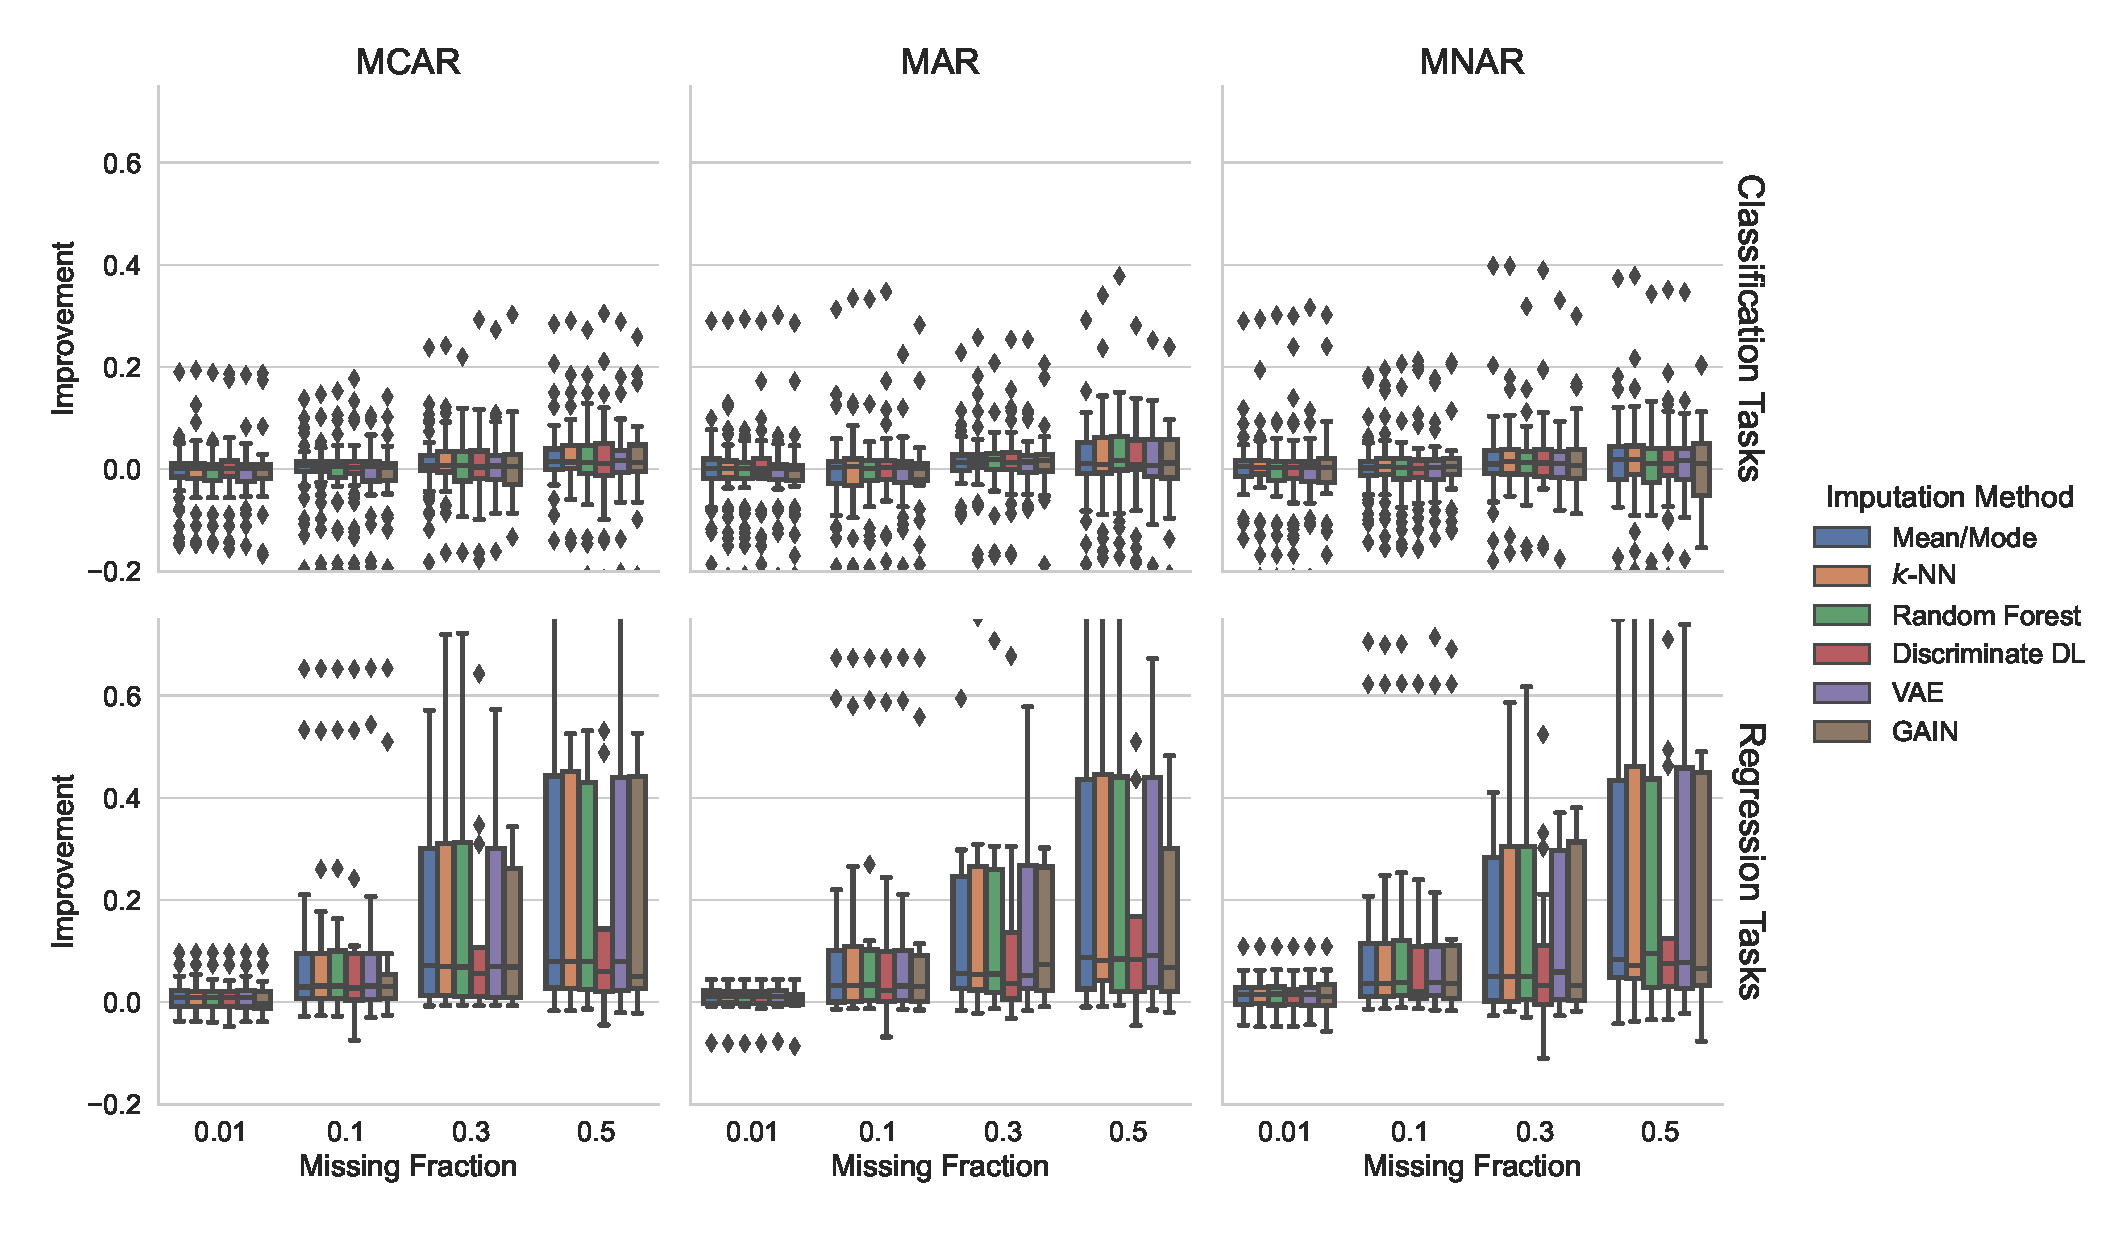
\includegraphics[width=1\columnwidth]{fully_observed_downstream_boxplot.eps}

	\caption[Downstream Ranks - Fully Observed]{Impact on downstream task of the six imputation methods trained on complete data. We plot the imputation method's rank against the missingness fraction. The columns of plots separate the changing missingness pattern, whereas the rows distinguish the results between categorical and numerical target columns. Overall, the classical ML methods and discriminative DL perform best.
    }
	\label{fig:fully_observed_downstream_boxplot}
\end{figure}

Figure \ref{fig:fully_observed_downstream_boxplot} visualizes the \textit{impact on downstream task} metric (Equation \ref{eq:impact}) in \textit{Scenario 1}. \arndt{hier ggf. in einem Satz nochmal zusammenfassen, wie die Berechnung erfolgt (sinngemäß).}

The impact of imputation seems mostly negligible if the proportion of missing values is only 1\%. However, for numeric columns, there are some outliers in the 20\% to 40\% improvement range with the MCAR and MAR patterns at 1\% missing values. With an increasing proportion of missing values we observe increasing improvements in the downstream performance in all types of missingness patterns. However, there are also some cases where downstream performance is degraded by imputation, which is mainly the case for categorical columns.

For categorical columns, improvements are mostly in the 0\% to 5\% range, and in case of 50\% missing values the upper quartile reaches the 5\% to 10\% range. The whiskers even indicate performance increases which go significantly beyond. Measured by the median, as an overall aggregation, Random Forest yields the best results for categorical columns. GAIN performs often similarly well or even better but also has more negative fluctuations.

The situation is different for regression tasks. Here, GAIN clearly yields the least improvements downstream. Even the Mean imputation is oftentimes significantly more beneficial for the downstream tasks. The VAE results are approximately on par with Mean imputation. In contrast, the classical ML and the discriminative DL approaches do outperform the other methods in most settings. However, when the missing values are MNAR there is no clear advantage except that the discriminative DL is superior at 50\% missing values.

Overall, the classical ML methods and discriminative DL perform best. As the proportion of missing values increases, we observe increasing improvements in all types of missingness patterns, along with higher variance, in downstream performance. In contrast to classification tasks, there are hardly any negative effects in regression tasks.

\subsubsection{Scenario 2: Training on Incomplete/Imputed Data}

\sebastian{Auch hier: variance wird größer, wenn fraciton steigt. Jetzt aber tendenziell verschlechterungen.. Wieder aber für Regression besser als für classification. Mit KNN/Forest beste cahnce auf verbesserung.}


\begin{figure}\centering
	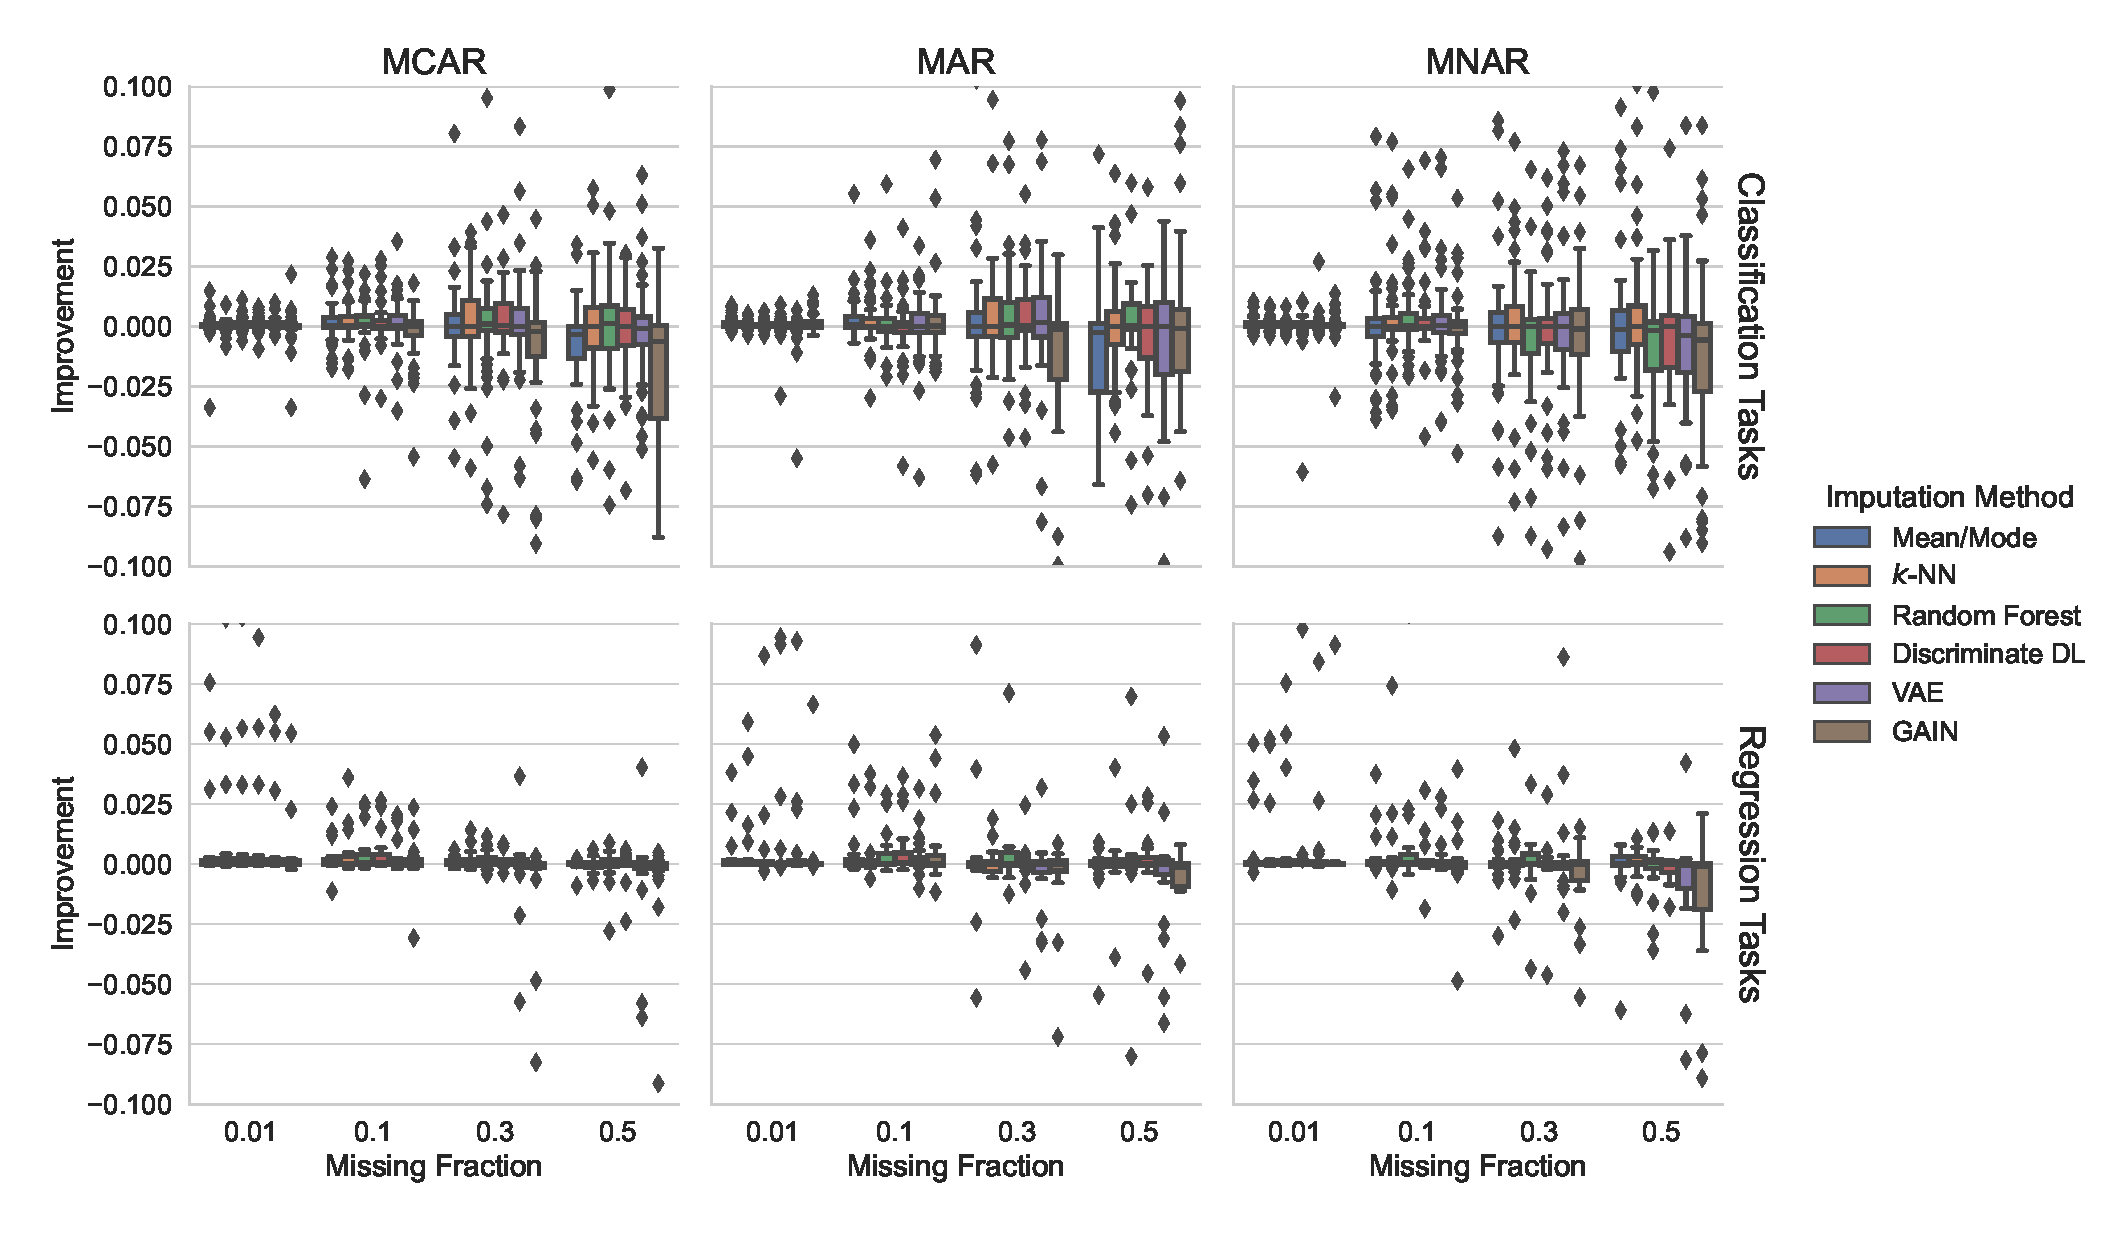
\includegraphics[width=1\columnwidth]{corrupted_downstream_boxplot.eps}

	\caption[Downstream Ranks - Corrupted]{Impact on downstream task of the six imputation methods trained on incomplete/imputed data. We plot the imputation method's rank against the missingness fraction. The columns of plots separate the changing missingness pattern, whereas the rows distinguish the results between categorical and numerical target columns. In regression tasks, no considerable improvements are achieved. In classification tasks, in contrast, we observe slightly positive effects in some settings but negative effects predominate in the harder settings.
    }
	\label{fig:corrupted_downstream_boxplot}
\end{figure}

Figure \ref{fig:corrupted_downstream_boxplot} illustrates the \textit{impact on downstream task} (Equation \ref{eq:impact_scenario2}) in \textit{Scenario 2} (training on incomplete/imputed data). Here, the different scaling of the y-axis must be taken into account, i.e. the relative improvements are significantly smaller compared to the first scenario. One reason for this is the different basis for calculating the relative values (see sections \autoref{sec:experiment_2} and \autoref{sec:scenario_2}). \arndt{@Sebastian vllt. magsts du das noch mit einem weiteren Satz ausführen?!} \sebastian{wüsste nicht wie, es gibt halt keine andere Basis..}

If weak positive effects seem to predominate in classification tasks at first, this tendency changes with increasing proportion of missing values (at 50\%) and increasing difficulty of the task (especially MNAR). The most negative results are produced by GAIN. However, the other methods also have major difficulties and often drift into negative ranges for the greater part as the tasks become more challenging.

In regression tasks, apart from a few outliers, there are no significant improvements. At the highest proportion of missing values (50\%) and greatest difficulty (MNAR), the results of the generative methods (VAE and GAIN) even turn predominantly negative.

In summary, no considerable improvements were achieved in regression tasks. In classification tasks, the picture is more mixed and the variance is higher. In some settings, there are slightly positive effects to note. In the difficult settings, however, the negative effects predominate.


\felix{
\begin{itemize}
\item in the conclusion we should relate the performance to the training and prediction time and comment on the (large) differences - for AutoKeras, a lot more tuning is performed and we don't know whether it would have worked as well with less tuning.
\item we should highlight the limitations of our results (only one column, maybe too simple)
\item we should highlight the main findings; as far as i can see this would be: a) classical methods perform best (on these simple (?) data sets) and b) downstream performance is improved by X \% in Y \% of the experiments (we can use the quantiles in the boxplots) whereas when the imputation methods are trained on incomplete data, we cannot expect improvements.
\end{itemize}
}
\arndt{consider Felix' points above in discussion}




\subsection{Training Time}

\begin{table}
	\centering
	\label{tab:time}
	\begin{tabular}{lrr}
		\toprule
		Imputation Method &  Training Time &  Relative Standard Deviation \\
		\midrule
		Mean/Mode &       0.005009 &                     0.656056 \\
		$k$-NN &      40.961577 &                     0.243020 \\
		Random Forest &     225.513999 &                     0.118707 \\
		Discriminative DL &    6285.017741 &                     0.424011 \\
		VAE &      71.685278 &                     0.107189 \\
		GAIN &     874.657293 &                     0.299608 \\
		\bottomrule
	\end{tabular}
	\caption{Training time for each imputation method in seconds. Training time is the mean overall experimental settings, experiments, and scenarios. The data set's size skews the standard deviation heavily, which is why we first compute the relative standard deviation for each imputation method on each data set separately and then average over the data sets.\felix{for knn the training time should be almost 0, right? maybe it would be good to have the inference/prediction times as well, if we have that? kNN should perform much worse here, and the winner should be RF, i'm assuming}}
\end{table}
